
\documentclass[12pt]{article}
\usepackage[french]{babel}
\usepackage[utf8x]{inputenc}
\usepackage{amsmath}
\usepackage{graphicx}
\usepackage[colorinlistoftodos]{todonotes} 
\usepackage{xcolor}
\usepackage{listings}

\definecolor{mGreen}{rgb}{0,0.6,0}
\definecolor{mGray}{rgb}{0.5,0.5,0.5}
\definecolor{mPurple}{rgb}{0.58,0,0.82}
\definecolor{backgroundColour}{rgb}{0.95,0.95,0.92}
\lstdefinestyle{CStyle}{
    backgroundcolor=\color{backgroundColour},   
    commentstyle=\color{mGreen},
    keywordstyle=\color{magenta},
    numberstyle=\tiny\color{mGray},
    stringstyle=\color{mPurple},
    basicstyle=\footnotesize,
    breakatwhitespace=false,         
    breaklines=true,                 
    captionpos=b,                    
    keepspaces=true,                 
    numbers=left,                    
    numbersep=5pt,                  
    showspaces=false,                
    showstringspaces=false,
    showtabs=false,                  
    tabsize=2,
    language=C
}

\begin{document}

\begin{titlepage}

\newcommand{\HRule}{\rule{\linewidth}{0.5mm}} % Defines a new command for the horizontal lines, change thickness here

\center % Center everything on the page
 

\textsc{\LARGE Ecole Polytechnique Universitaire de Lille}\\[1.5cm] % Name of your university/college
\textsc{\Large Projet IMA3}\\[0.5cm] % Major heading such as course name
\textsc{\large }\\[0.5cm] % Minor heading such as course title


\HRule \\[0.4cm]
{ \huge \bfseries Rapport Projet SimulPhys }\\[0.4cm] % Title of your document
\HRule \\[1.5cm]
 


\begin{minipage}{0.4\textwidth}
\begin{flushleft} \large
Corto \textsc{Callerisa} % Your name

Alex \textsc{Lagneau} % Supervisor's Name

Clément \textsc{Hue} % Supervisor's Name
\end{flushleft}
\end{minipage}
~
\begin{minipage}{0.4\textwidth}
\begin{flushright} \large
Sébastien \textsc{Dardenne} % Supervisor's Name
Quentin \textsc{Normand} % Supervisor's Name
\end{flushright}
\end{minipage}\\[2cm]


% If you don't want a supervisor, uncomment the two lines below and remove the section above
%\Large \emph{Author:}\\
%John \textsc{Smith}\\[3cm] % Your name

%----------------------------------------------------------------------------------------
%	DATE SECTION
%----------------------------------------------------------------------------------------

{\large{Soutenance le 4 juin 2019}}\\[2cm] % Date, change the \today to a set date if you want to be precise
%{ \large \today}\\[2cm] % Date, change the \today to a set date if you want to be precise

%----------------------------------------------------------------------------------------
%	LOGO SECTION
%----------------------------------------------------------------------------------------


\includegraphics[scale=0.4]{logo.png} % Include a department/university logo - this will require the graphicx package
 
%----------------------------------------------------------------------------------------
 
\vfill % Fill the rest of the page with whitespace


\end{titlepage}
\clearpage \vspace*{\fill} \begin{center} \begin{minipage}{\textwidth} \centering{\tableofcontents} \end{minipage} \end{center} \vfill % equivalent to \vspace{\fill} \clearpage
\newpage
\addcontentsline{toc}{part}{Introduction}
\section*{Introduction}
Dans un contexte économique où pour chaque entreprise, réduire les coûts de conception et de production est nécessaire afin d’être compétitif sur le marché, la simulation physique sur ordinateur s’impose comme un outil extraordinaire pour faire des premiers prototypes sans avoir à dépenser une fortune en crash-test. C’est dans ce contexte que nous avons choisi de réaliser un simulateur configurable de processus physique destiné à la conception et au développement de systèmes automatisés, s’implémentant aussi dans le concept d’entreprise 4.0.

\section{Analyse du projet}

Tout d’abord, nous avons dû définir les limites du sujet. C’est pourquoi dans un premier temps nous avons recherché quelles sont les solutions existantes (RobotDk, Delmia…)  et étudié les différents systèmes présents à Polytech (Ascenseur, Tri de colis, Train 2D...).Nous avons ensuite choisi un système à reproduire (l’ascenseur) afin de le modéliser dans notre application.
\newline
Les objectifs sont alors de modéliser l’ascenseur avec une visualisation en 3D, et de permettre à ce modèle de communiquer avec un terminal distant.
\newline
\newline
Nous avons étudié plusieurs possibilités pour effectuer la modélisation : Unreal Engine, Unity, Godot,… Chacun présentant avantages et inconvénients.
La facilité de prise en main et la portabilité sur différentes plateformes nous ont fait choisir Godot. De plus, Godot ne permet pas seulement une visualisation, mais possède également un moteur physique intégré performant nous permettant désormais de se concentrer sur la réalisation du modèle et sur la communication.
\newline
\newline
Nous avons également étudié différentes méthodes de communication : mémoire partagée, Pipe, TCP/IP, UDP… 
Nous avons choisi le protocole UDP car il est simple d’implémentation ce qui permet d’avoir une commande sous plusieurs formes (Godot, python, netcat sous linux). De plus, il est rapide ce qui permet un contrôle précis de la simulation.. 
\newpage

\section{Simulation}
Nous avons décidé de simuler pour notre premier système un ascenseur. Le système possède 6 niveaux, est contrôlé par des boutons situés dans l’ascenseur et sur chaque palier pour l’appeler et comporte des capteurs pour le situer. Il est constitué des objets suivants : une cage d’ascenseur avec des portes coulissantes, des capteurs de présence et des boutons poussoir.
\subsection{La cage d’ascenseur :}
\newline
Le contrôle de l’ascenseur se fait par état : l’appui sur un bouton le met sur l’état “haut” ou “bas” pour le faire monter ou descendre; les capteurs de présence lui indiquent à quel étage il se situe puis il change son état sur “stop” quand il arrive à l’étage désiré.
L’ascenseur est géré par le script “CageAscenseur.gd” qui contient la fonction \_process servant à modifier sa position dans l’espace en fonction de son état.
\newline
\begin{center}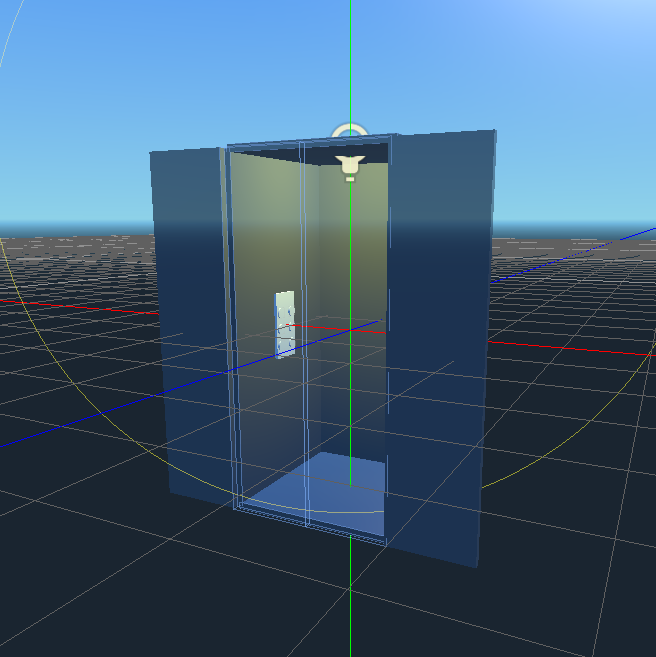
\includegraphics[scale=0.4]{asc.PNG}\end{center}
\newline
\newline
\subsection{Les capteurs :}
\newline
Les capteurs utilisent l’objet RayCast de Godot, cet objet peut détecter si un objet est positionné devant lui grâce à sa fonction “is\_colliding()”. On peut donc savoir quand l’ascenseur passe devant et, grâce à la fonction “update” de l’ascenseur, il peut lui indiquer à quel niveau il se situe. Si le capteur actionné est celui de l’étage désiré, la fonction update change l’état de l’ascenseur sur “stop”.
\newline
\begin{center}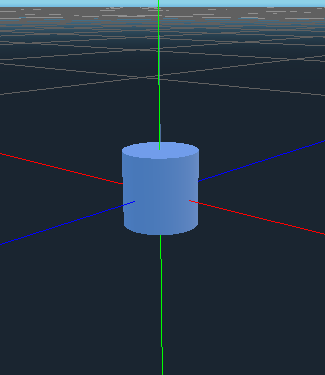
\includegraphics[scale=0.6]{capteur.PNG}\end{center}
\newline
\newline
\subsection{Les boutons :}
\newline
Le système est composé de 6 niveaux donc l’ascenseur contient 6 boutons et à chaque niveau se trouve un boîtier contenant un bouton pour appeler l’ascenseur. A l’appui du bouton le script appelle la fonction “appel” de l’ascenseur avec comme paramètre l’étage de destination; l’ascenseur va modifier son état en fonction de l’étage appelé.
\newline
\begin{center}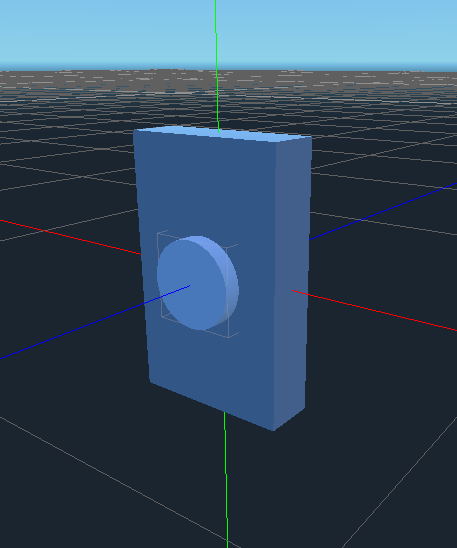
\includegraphics[scale=0.4]{bouton.PNG}\end{center}
\newline
En plus d’effectuer ces actions, chaque appui sur un bouton ou changement d’état d’un capteur est notifié dans la commande et peut être affiché dans une invite de commande.

\newpage
\section{Communication}

Après avoir étudié différentes méthodes de communication nous avons choisi d’utiliser le protocole UDP. En effet ce protocole permet une communication en réseau rapide ce qui permet une commande très réactive. De plus cela permet d’avoir une interface uniforme pour se connecter à la simulation, les bibliothèques UDP étant intégrées dans de nombreux langages. 
\newline
\newline
La communication se fait entre 3 parties indépendantes s’inspirant du modèle MVC (Modèle-vue-contrôleur). La commande s’effectue depuis un script avec une invite de commande, la vue est la fenêtre de simulation de Godot qui héberge aussi le modèle.
\subsection{Transmission :}
\newline
Nous avons défini et implémenté un protocol de communication simple :
\newline
\textbf{‘+-*/’} \guilsinglleft{}var\guilsinglright{} value : permet respectivement d’augmenter, diminuer, multiplier ou diviser une variable par une valeur.
\newline
\textbf{get \guilsinglleft{}var\guilsinglright{} :} demande la valeur courante de la variable \guilsinglleft{}var\guilsinglright{}
\newline
\textbf{set \guilsinglleft{}var\guilsinglright{} value :} modifie de façon absolue \guilsinglleft{}var\guilsinglright{}
\newline
\newline
Il y a aussi des fonctions spécifiques à la simulation de l’ascenseur : 
\newline
\textbf{etage \guilsinglleft{}num\guilsinglright{} :} permet de déplacer l’ascenseur à l’étage \guilsinglleft{}num\guilsinglright{} compris entre 0 et 5.
\newline
\textbf{open :} ouvre les portes de l’ascenseur
\newline
\textbf{close :} ferme les portes de l’ascenseur
\newline
\newline
Il y a également des fonctions utilisées par la commande :
\newline
\textbf{record\guilsinglleft{}nom\_script.cmd\guilsinglright{} :} démarre l’enregistrement des commandes dans le fichier \guilsinglleft{}nom\_script.cmd\guilsinglright{}
\newline
\textbf{playback \guilsinglleft{}nom\_script.cmd\guilsinglright{} :} rejoue la séquence de commande sauvegardée dans \guilsinglleft{}nom\_script.cmd\guilsinglright{}
\newline
Le port et l’adresse ip du serveur de destination sont des arguments optionnels du script.
\newline
Il est possible d’ouvrir plusieurs fenêtres de commandes sur des postes différents.
\newline
L’implémentation d’un terminal spécifique à la commande augmente l’ergonomie pour l’utilisateur grâce aux fonctions d'autocomplétion et d’historique.

\begin{center}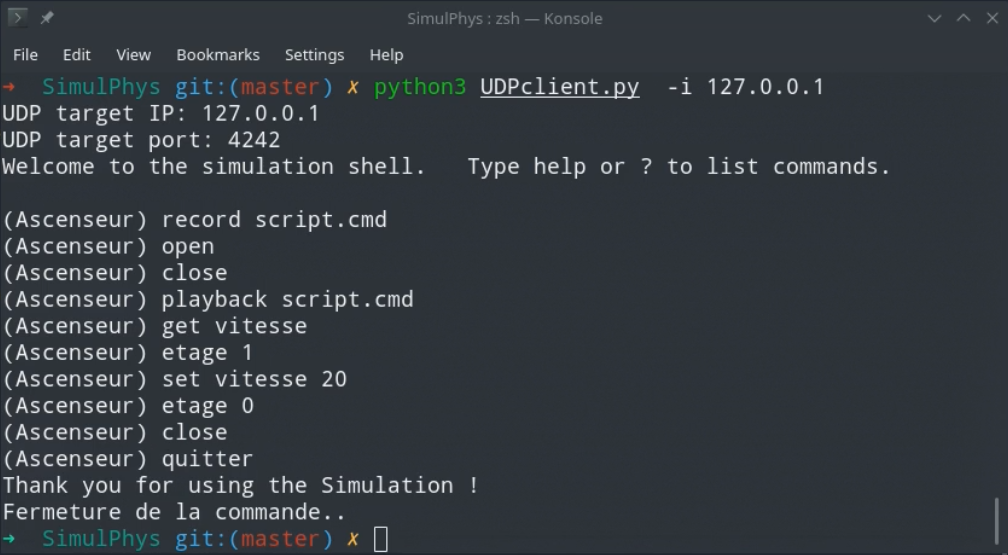
\includegraphics[scale=0.4]{commande.png}\end{center}

\subsection{Réception :}

Les messages envoyés par la commande sont reçus et traités dans la simulation par Godot. 
\newline
A chaque frame le programme scrute l’arrivée d’un message et si un message est reçu celui-ci est “tokenizé”, c’est à dire décomposé en “tokens” permettant de comprendre la commande. Exemple  : la commande “+ vitesse 10” contient les tokens ‘+’ ‘vitesse’ et ‘10’. Le programme peut donc comprendre qu’il doit augmenter la vitesse de l’ascenseur de 10 unité.
\newline
La simulation est ensuite mise à jours et un message est envoyé à la partie réception.
Il est également possible d’interagir avec les boutons de la simulation pour appeler l’ascenseur. Un message indiquant la provenance et l’étage d’appel est envoyé.
\newline
Un menu permettant de configurer les paramètres d’envoi et de réception est inclus pour l’ergonomie utilisateur.
\newpage
\subsection{Réponse :}

Le système est surveillé en temps réel et renvoie son état par communication UDP à chaque réception de commande. Ces réponses sont affichés dans une console et peuvent être exportés en format CSV si l’argument -e ou --export est passé au script.
\newline
Le temps est ajouté à chaque ligne avec une précision d’un millionième de seconde afin de faciliter l’analyse de la réponse du système. 
\newline
Il est possible d’ouvrir une fenêtre de réponse sur plusieurs postes simultanément.

\begin{center}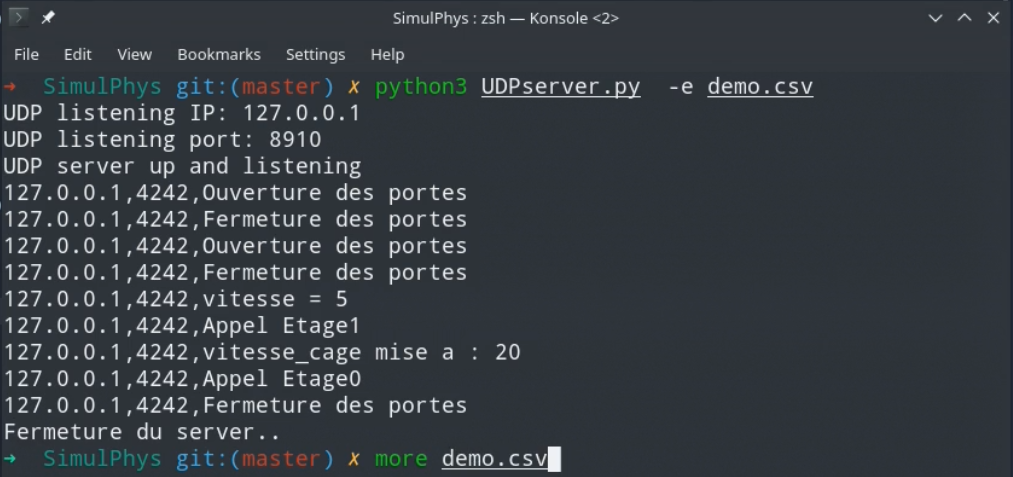
\includegraphics[scale=0.4]{reception.png}\end{center}

\addcontentsline{toc}{part}{Conclusion}

\section*{Conclusion :}
Au cours de ce projet nous avons développé nos connaissances en informatique, particulièrement en modélisation et réseau, en réalisant un simulateur de processus physique en collaboration. 
\newline
\newline
Nous avons procédé en suivant une démarche de projet. D’abord nous avons défini le sujet en précisant le besoin, ses limites et l'environnement  d’implémentation. Nous avons ensuite fait une recherche documentaire afin d’étudier les solutions possibles pour la communication et la simulation ainsi que l’interface. Nous divisé le travail en deux grandes parties : Simulation et Commande. Finalement nous avons implémenté un simulateur d’ascenseur en Godot, avec une commande séparée codé en python et utilisant le protocole UDP.
\newline
\newline
Pour la suite notre objectif est d’implémenter un système plus complexe.
\end{document}